\documentclass[12pt,oneside]{book}
\usepackage[utf8]{inputenc}
\usepackage[T1]{fontenc}
\usepackage{lmodern}
\usepackage[slovak]{babel}
\usepackage{graphicx}
\usepackage{anysize}
\usepackage{hyperref}
\usepackage{appendix}

\ifpdf
\pdfcompresslevel=9
\else
\usepackage{graphicx}
\fi

\def\mftitle{Domáce účtovníctvo}
\def\mfthesistype{Bakalárska práca}
\def\mfauthor{Peter Kotulič}
\def\mfadvisor{Mgr. Ján Kľuka, PhD.}
\def\mfplacedate{Bratislava, 2013}

\hypersetup{
    bookmarks=true,         % show bookmarks bar?
    unicode=true,          % non-Latin characters in Acrobat’s bookmarks
    pdftoolbar=true,        % show Acrobat’s toolbar?
    pdfmenubar=true,        % show Acrobat’s menu?
    pdffitwindow=false,     % window fit to page when opened
    pdfstartview={FitH},    % fits the width of the page to the window
    pdftitle={\mftitle},    % title
    pdfauthor={\mfauthor},     % author
    pdfsubject={Subject},   % subject of the document
    pdfcreator={\mfauthor},   % creator of the document
    pdfkeywords={accounting, finance, framework, MVC, CakePHP}, % list of keywords
    pdfnewwindow=true,      % links in new window
    colorlinks=true,       % false: boxed links; true: colored links
    linkcolor=blue,          % color of internal links
    citecolor=green,        % color of links to bibliography
    filecolor=cyan,      % color of file links
    urlcolor=blue           % color of external links
}

\usepackage{listings}
\usepackage{color}

\definecolor{dkgreen}{rgb}{0,0.6,0}
\definecolor{gray}{rgb}{0.5,0.5,0.5}
\definecolor{mauve}{rgb}{0.58,0,0.82}

\lstset{frame=tb,
  language=php,
  aboveskip=3mm,
  belowskip=3mm,
  showstringspaces=false,
  columns=flexible,
  basicstyle={\small\ttfamily},
  numbers=none,
  numberstyle=\tiny\color{gray},
  keywordstyle=\color{blue},
  commentstyle=\color{dkgreen},
  stringstyle=\color{mauve},
  breaklines=true,
  breakatwhitespace=true
  tabsize=3
}

\renewcommand\baselinestretch{1.3} 

\marginsize{3.5cm}{2cm}{2.5cm}{2.5cm}

\ifx\pdfoutput\undefined\relax\else\pdfinfo{ /Title (\mftitle) /Author (\mfauthor) /Creator (PDFLaTeX) } \fi

\begin{document}

\frontmatter

\thispagestyle{empty}

\noindent
\begin{minipage}{1\textwidth}
\begin{center}
\large\bf UNIVERZITA KOMENSKÉHO V BRATISLAVE\\
FAKULTA MATEMATIKY, FYZIKY A INFORMATIKY\\
\end{center}
\end{minipage}

\vfill
\begin{minipage}{0.8\textwidth}
\begin{center}
\LARGE\bf\sc\mftitle \\
\smallskip
\large\bf\mfthesistype
\end{center}
\end{minipage}
\vfill
\vspace{7\baselineskip}
{\large\bf 2013 \hfill \mfauthor}
\eject


\thispagestyle{empty}

\noindent
\begin{minipage}{1\textwidth}
\begin{center}
\large\bf UNIVERZITA KOMENSKÉHO V BRATISLAVE\\
FAKULTA MATEMATIKY, FYZIKY A INFORMATIKY
\end{center}
\end{minipage}
\vfill
\begin{minipage}{0.8\textwidth}
\begin{center}
\LARGE\sc\mftitle \\
\smallskip
\large\bf\mfthesistype
\end{center}
\end{minipage}
\vfill
\noindent
  \begin{tabular}{ @{} l l  }
	Študijný program: 		&Aplikovaná informatika \\
	Študijný odbor: 		&2511 Aplikovaná informatika\\
	Školiace pracovisko: 	&Katedra aplikovanej informatiky\\
	Školiteľ: 			&\mfadvisor \\
  \end{tabular}

\vspace{3\baselineskip}
\noindent{\large\bf\mfplacedate \hfill \mfauthor\par}
\eject


\thispagestyle{empty}

\noindent
\begin{minipage}{1\textwidth}
\begin{center}
Univerzita Komenského v Bratislave\\
Fakulta Matematiky, Fyziky a Informatiky
\smallskip
\end{center}
\end{minipage}
\hrule

\begin{center}
\centerline{\Large \bf Zadanie}
\end{center}

{\bf Meno a priezvisko študenta:} \mfauthor \\

{\bf Študijný program:} aplikovaná informatika \\

{\bf Typ záverečnej práce:} bakalárska \\

{\bf Jazyk záverečnej práce:} slovenský \\

{\bf Názov:} \mftitle \\

{\bf Cieľ práce:} Navrhnúť a implementovať webovú aplikáciu umožňujúcu používateľom udržiavanie prehľadu o príjmoch a výdavkoch ich rodinných rozpočtov v minulosti a jednoduché formy plánovania do budúcnosti. Prispôsobiť najčastejšie potrebné funkcie mobilnému použitiu. Využiť framework pre vývoj webových aplikácií, návrhové vzory a rigorózne testovanie. \\

{\bf Školiteľ:} \mfadvisor \\

\bigskip

\hfill\hbox{ V Bratislave 22. októbra 2012} \hfill\hbox{ \begin{tabular}{c} \\ doc. RNDr. Mária Markošová, PhD.\\ gestor št. programu \end{tabular}} \\

\bigskip

\hfill\hbox{ \begin{tabular}{c} \\ Peter Kotulič \\  študent \end{tabular}} \hfill\hbox{ \begin{tabular}{c} \\ Mgr. Ján Kľuka, PhD. \\ vedúci, resp. školiteľ \end{tabular}}

\eject


\section*{Abstrakt}
KOTULIČ, Peter: \mftitle. [\mfthesistype] – Univerzita Komenského v Bratislave. Fakulta matematiky, fyziky a informatiky; Katedra aplikovanej informatiky. – Školiteľ: Mgr. Ján Kľuka, PhD.. 

TODO

{\bf Kľúčové slová: účtovníctvo, financie, framework, MVC, CakePHP}

\section*{Abstract}
KOTULIČ, Peter: Home accounting software. [Bachelor thesis] – Comenius University in Bratislava. Faculty of Mathematics, Physics and Informatics; Department of Applied Informatics. – Supervisor: Mgr. Ján Kľuka, PhD.. 

TODO

{\bf Keywords: accounting, finance, framework, MVC, CakePHP}

\eject

{~}\vspace{12cm}

\noindent
\begin{minipage}{0.25\textwidth}~\end{minipage}
\begin{minipage}{0.68\textwidth}
Čestne prehlasujem, že som túto bakalársku prácu vypracoval(a) samostatne s použitím citovaných zdrojov.

\bigskip\bigskip

V Bratislave 31. mája \hfill\hbox to 6cm{\dotfill}
\end{minipage}
\vfill\eject

\tableofcontents

\newpage


\mainmatter

\chapter{Úvod}\label{chap:intro}

\section{Motivácia}
Pri tvorbe tejto práce ma najviac ovplyvnila aktuálna situácia v našej spoločnosti, ktorá je čím ďalej, tým viac konzumne zameraná. Nakupujeme oveľa viac ako v minulosti. A nejde len o potrebné veci. A čím viac vecí nakúpime, tým menší prehľad v nich máme. A tak nakupujeme ešte viac. Tento konzumný spôsob života vplýva najviac na našu peňaženku. A rovnako ako máme problém vyznať sa vo veciach ktoré nakupujeme, rovnako vzniká problém vyznať sa aj v našich financiách. A toto by som rád vyriešil. Verím tomu, že čím viac budeme mať svoje financie pod kontrolou, tým lepšie sa nám bude žiť. Čím lepšie budeme vedieť na čo míňame, tým ľahšie sa nám bude dať naplánovať na ktorých veciach môžeme ušetriť. Mať prehľad a začať spravovať svoje domáce účtovníctvo je tým prvým krokom, ktorý musíme urobiť.

Ďalšou významnou motiváciou k tvorbe tejto práce bola pre mňa túžba naučiť sa niečo nové. Niečo, čoho znalosti mi veľmi dobre poslúžia aj pri mojich budúcich projektoch. V tomto prípade ide o použitie \emph{frameworku} (vývojového rámca) na tvorbu webových aplikácii. Bude sa na ňom zakladať celá moja aplikácia na domáce účtovníctvo.   

\section{Ciele práce}
Hlavným cieľom tejto práce je vytvoriť webovú aplikáciu Domáce účtovníctvo na jednoduchú a prehľadnú správu osobných (domácich?) financií. Keďže je už podobných aplikácii dosť veľa, mojím plánom nebude urobiť len ich jednoduchú kópiu. Budem sa snažiť porovnať tieto existujúce aplikácie, vyhodnotiť ich klady a zápory, a z každej si zobrať len to najlepšie, čo implementujem do mojej výslednej aplikácie. Zamerať sa chcem taktiež aj na jednoduché a prehľadné grafické rozhranie aplikácie, v ktorom sa používateľ bude vedieť orientovať po pár kliknutiach myšou. Toto je jedna z vecí, ktorú by už existujúci podobné aplikácie mali prepracovať. Pri ich skúmaní sa mi často stávalo, že som nevedel a musel dlho hľadať ako vykonať určitú akciu. A toto sa pri aplikáciách, ktoré sú určené bežným používateľom nesmie stávať. Podobným jednoduchým a prehľadným štýlom bude spravená aj mobilná verzia aplikácie. V jednoduchosti je krása. A tak myslím, že je zbytočné robiť prekomplikovanú aplikáciu s \uv{milión} funkciami, keď ju používateľ po piatich minútach vypne, lebo sa v nej nevyzná.


\chapter{Východiská}\label{chap:background}
V tejto časti práce sa budem snažiť opísať východiská, ktoré ma inšpirovali a pomohli mi pri tvorbe bakalárskej práce. Okrem opisu základnej teórie potrebnej na realizáciu práce pôjde aj o prehľad funkčných požiadaviek na výslednú aplikáciu.

Taktiež spravím prehľad už implementovaných, podobných riešení na správu domáceho účtovníctva. Budem sa zaoberať tromi hlavnými typmi aplikácií. Pôjde o webové, mobilné a desktopové aplikácie na správu a prehľad financií v domácnosti. Mojou snahou je zhrnúť základné vlastnosti a funkcionalitu týchto aplikácií, z každej si zobrať to najlepšie a implementovať to do mojej práce v čo najväčšej miere.

Ďalšiu časť tejto kapitoly bude tvoriť popis Model–view–controller architektúry(MVC) \cite{UvodMVC}\ , ktorá bude s pomocou frameworku CakePHP použitá aj v mojej práci. V súčasnosti ide o jeden z najobľúbenejších spôsobov tvorby aplikácií. Keďže som už spomenul aj framework v ktorom budem robiť aplikáciu, rád by som časť tejto kapitoly venoval aj jemu.
Nakoniec by som sa rád pozrel a priblížil aj tému návrhových vzorov, ktoré takáto práca bude vyžadovať.\newpage



\section{Použité webové technológie}
\subsection{HTML a CSS}
HTML \cite{HTML}\ je skratka pre HyperText Markup Language. Je to najpoužívanejší značkovací jazyk na zápis hypermediálnych dokumentov, ktorý používame pri tvorbe web stránok. Štruktúru HTML dokumentu určuje definícia typu (Document Type Definition; DTD). Táto definícia určuje množinu značiek, ktoré môžu byť použité v dokumente. 

Aktuálna verzia tohto jazyka je HTML 5 \cite{HTML5}\ . Táto verzia priniesla mnoho výhod. Okrem tagu video, ktorý by sa mal stať novým štandardom na prezeranie videí a filmov na webe ide hlavne o nové štrukturálne elementy.
 
Element \texttt{div} teraz môže byť nahradený presnejšie definovanými elementmi ako sú \texttt{header}, nav, section, article, aside a footer. Na jednej strane to pomáha k prehľadnejšiemu kódu a na druhú stranu aj koncovému používateľovi pri jednoduchšom pohybe na stránke. Napríklad môže ísť o rýchle preskočenie navigácie alebo jednoduchší pohyb medzi rôznymi článkami.

Ďalšou novinkou sú nové atribúty ktoré môžeme využiť pri formulároch a inputoch. Pre mňa poslednou dôležitou výhodou HTML 5 ktorú by som rád spomenul je použitie Inline SVG(Scalable Vector Graphics) . Ide o vektorovú grafiku ktorú používa aj mnou neskôr spomínaná javascriptová Highcharts knižnica.

CSS \cite{CSS21}\ (Cascading Style Sheets - kaskádové štýly) je štýlovací jazyk, ktorý popisuje ako budú zobrazené stránky, ktoré boli napísané v (X)HTML. CSS umožňujú vizuálne formátovať webové dokumenty. Vytvárame tak štruktúrované dokumenty v ktorých oddeľujeme obsah dokumentu(HTML) od jeho vzhľadu(CSS). Hlavné z výhod použitia CSS su prehľadnejší kód, menšia dátová náročnosť a jednoduchá zmena formátovania určitých elementov na celej stránke bez nutnosti formátovania každého elementu zvlášť. 

\subsection{CakePHP} 
CakePHP \cite{CakePHP}\ je open source webový framework určený na vývoj webových aplikácií v programovacom jazyku PHP verzie 4 a 5. Tento framework vznikol už v roku 2005 ako reakcia na veľmi obľúbený a úspešný framework Ruby on Rails. Framework CakePHP je postavený na softwareovej architektúre Model-view-controller, ktorý bližšie opisujem v kapitole 2.4.


\subsection{Highcharts plugin} 
Tento plugin \cite{HighchartsPlugin}\ pre framework CakePHP využíva niektoré skvelé možnosti knižnice pre tvorbu grafov Highcharts. Hlavnou výhodou tejto knižnice je, že je kompletne napísaná v JavaScripte. Pre jej fungovanie nie sú potrebné žiadne client side pluginy akými sú napríklad Java alebo Flash. Knižnica Highcharts funguje vo všetkých moderných webových prehliadačoch a nerobia jej problém ani tie mobilné. Ako na Androide, tak aj na iOS. Použitý plugin pre CakePHP je stále vo vývoji, a preto zatiaľ neponúka všetky výhody Highcharts. Základná funkcionalita ktorú poskytuje však plne postačuje na využitie v mojej aplikácii.

\section{Existujúce riešenia}
Pred začatím tvorby svojej aplikácie som urobil prehľad podobných existujúcich riešení. Rozdelil som ich do troch kategórií. Webové aplikácie, desktopové aplikácie a mobilné aplikácie.
Na začiatok by som rád uviedol, že všetky ďalej spomínané aplikácie spĺňali určitú základnú funkcionalitu, ktorú od aplikácie na prehľad rozpočtu berieme za samozrejmú.
\begin{itemize}
\item{pridávanie, editovanie a mazanie jednorazových príjmov a výdavkov}
\item{pridávanie, editovanie a mazanie opakovaných príjmov a výdavkov}
\end{itemize}

\subsection{Webové aplikácie}
\subsubsection{Budget Pulse \cite{BudgetPulse}\ }

Webová aplikácia Budget Pulse ponúka jednoduchú administráciu a prehľady transakcií. Trochu horšie je spracované menej prehľadné pridávanie výdavkov a príjmov. Jednou za základných funkcií tejto aplikácie je vytvorenie novej transakcie. V následnom menu si používateľ vyberie či ide o príjem alebo výdavok, určí jeho kategóriu, popis, sumu, množstvo, konto(účet) ktoré chce použiť, dátum transakcie a zadá prípadné opakovania transakcie. Zaujímavou funkciou v tejto aplikácii je možnosť rozdelenia transakcie na menšie časti a ich priradenie do rôznych kategórií. Budget Pulse taktiež ponúka vytvorenie viacerých kont pod jedným účtom. Ďalšou užitočnou funkciou je import a export dát z aplikácie. Za spomenutie taktiež stojí možnosť určenia osobných cieľov. Používateľ si nastaví sumu, ktorá sa mu napríklad raz za mesiac odčíta z konta a priradí k určitému osobnému cieľu, na ktorý si chce našetriť. Na jednoduchý prehľad medzi transakciami a kategóriami využíva aplikácia okrem klasického tabuľkového zobrazenia kategórií v čase aj grafy. Jednoduchý koláčový graf kategórií a stĺpcový graf kategórií za určité obdobie.



\subsubsection{Buxfer \cite{Buxfer}\ }

Druhá podobná webová aplikácia ktorú som testoval bola Buxfer. Hneď na prvý pohľad ma zaujal oveľa prepracovanejší a prehľadnejší dizajn ako pri Budget Pulse. Hlavne veľmi dobre spracovaná hlavná stránka. Zobrazuje 4 panely. Aktuálny stav účtu, výdavky za posledný mesiac zobrazené podľa kategórií koláčovým grafom a taktiež stĺpcovým grafom. Tieto grafy sa dajú v menu reports filtrovať aj podľa iného časového rozmedzia. Na poslednom panely sa nachádzajú pripomienky o budúcich výdavkoch. Pri transakciách nájdeme ich tabuľkové zobrazenie s popisom, sumou, tagmi, účtom a dátumom transakcie. Zaujímavou funkcie je prehľad požičaných peňazí. Pri pridávaní transakcií označujeme či ide o príjem, výdavok, transfer alebo refund. Do aplikácie môžeme taktiež nahrávať výpisy z banky. Za zmienku stojí aj vypočítavanie prehľadov do budúcna na základe predchádzajúcich príjmov a výdavkov.


\subsection{Desktopové aplikácie}
\subsubsection{RQ Money \cite{RQMoney}\ }

Jedinou desktopovou aplikáciou ktorá sa mi páčila a stála za otestovanie bolo RQMoney od slovenského autora. Aplikácia je vytvorená v Delphi. V porovnaní s predchádzajúcimi aplikáciami je RQMoney oveľa komplexnejšia a ponúka oveľa väčšiu funkcionalitu. V tomto sa dosť odlišuje od mojej webovej aplikácie Domáce účtovníctvo. Tá ma za cieľ prehľadnosť a jednoduchosť. 

RQMoney ponúka klasickú evidenciu príjmov, výdavkov a presunov. Používateľovi sú dostupné rôzne typy filtrov a radení podľa vlastného výberu. Užitočná funkcia je plánovanie transakcií s možnosťou prezerania platobného kalendára. S tým súvisí aj možnosť porovnania plánovaných a skutočných transakcií za mesiac. Štatistiky ponúkajú podrobné prehľady za rôzne časové obdobia vďaka tabuľkám a grafom. Používateľ môže v aplikácii použiť vlastné SQL príkazy. RQMoney obsahuje aj prehľadné tlačové zostavy a exporty tabuliek do MS Excel. Rovnako je možné exportovať aj grafy. 

\subsection{Mobilné aplikácie}
Zaoberal som sa len aplikáciami pre systém Android
\subsubsection{Easy Money - Android \cite{EasyMoney}\ }

Prvá aplikácia pre Android ktorú som testoval bola Easy Money. Ponúka rôzne typy účtov. Napríklad cash, kreditná karta, účet v banke. Pri pridávaní transakcií určujeme jej názov, cenu, kategóriu, dátum, či ide o príjem alebo výdavok a opakovanie. Okrem toho máme možnosť rozdeliť transakciu do viacerých kategórií a taktiež určiť, že ide len o prevod medzi účtami. 

V prehľadoch nám aplikácia ponúka zobrazenie príjmov alebo výdavkov podľa kategórií v stĺpcových grafoch. Okrem nich aj denne porovnanie príjmov a výdavkov a tiež ich mesačný zoznam a sumy za konkrétne mesiace. Ďalšou užitočnou vlastnosťou je pripomienkovač platenia faktúr a účtov. Zaujímavou funkciou je aj nastavenie mesačného rozpočtu a prehľad jeho využitia počas mesiaca. Easy Money podporuje import a export do QIF a CSV.  Medzi transakciami môže používateľ prehľadávať pomocou keywords.

\subsubsection{Money Lover - Android \cite{MoneyLover}\ }

Money Lover je najprehľadnejšia a najintuitívnejšia mobilná aplikácia, ktorú som testoval. Obsahuje jednoduché pridávanie transakcií pri ktorom určujeme či ide o príjem, výdaj, pôžičku alebo dlh. Potom vypĺňame polia názov, kategória, suma, poznámka, dátum, účet a prípadne nastavenie opakovania. Pri opakovaniach sa nedá nastaviť konkrétny dátum, ale len začiatok alebo koniec týždňa, pripadne mesiaca. Ako je možné už vidieť z vyplnených polí, môžeme používať rôzne typy účtov. Transakcie môžeme prehliadať v tabuľkových prehľadoch s možnosťou triedenia podľa dátumov, kategórií alebo príjmu a výdavkov. Koláčový graf kategórií za určité obdobie je už samozrejmosť. Aplikácia obsahuje aj menej zvyčajné funkcie ako je správa dlhov, prepočet meny, výpočet vrcholu, vyhľadanie bankomatu, banky a počítanie úroku. Zaujímavou funkciou je aj sprievodca pri nastavení aplikácie, ktorý by sa zišiel hlavne pri ostatných menej prehľadných aplikáciách. 

\subsubsection{Expense Manager - Android \cite{ExpenseManager}\ }

Poslednou Android aplikáciou ktorú som testoval bol Expense Manager. Klasicke pridávanie príjmov a výdavkov ma táto aplikácia vylepšené o možnosť prednastavenia predvypĺňaných polí. Ponúka taktiež možnosť pridávania opakujúcich sa transakcií. Na dopredu určené opakujúce sa obdobie má používateľ možnosť nastaviť rozpočet. 

Prehľad v transakciách ponúkajú koláčové a stĺpcové grafy príjmov alebo výdavkov triedených podľa kategórií a podľa mesiacov. Podkategórie si tiež môžeme zobraziť na koláčovom alebo stĺpcovom grafe. Graf je možné si vytvoriť aj zadaním vlastných kritérií(dátum od/do, príjem, výdavok, rozdiel, typ grafu).
Expense Manager ponúka ešte aj ďalšie možnosti ako je kalkulačka, prepočet meny, výpočet sprepitného, výpočet zľavy a dane alebo výpočet splatenia dlhov na kreditnej karte.

\subsection{Porovnanie s mojimi cieľmi}
Mojim hlavným cieľom je vytvoriť prehľadnú a užívateľsky jednoducho ovládajúcu sa aplikáciu. Všetky spomenuté podobné riešenia sa to tiež snažili splniť. Nie každému sa to však podarilo. Väčšina z aplikácií obsahovala okrem základnej funkcionality aj možnosti, ktoré bežný používateľ asi nikdy nevyužije. To by nevadilo, pokiaľ by tým aplikácia nestrácala na prehľadnosti. Bežný používateľ nemá čas a chuť zisťovať a učiť sa nanovo ovládať aplikáciu. Je zvyknutý na určité ovládacie prvky a ich prehľadné rozloženie. Napríklad pri aplikácii Budgetpulse je problém vykonať aj tú najzákladnejšiu akciu akou je pridanie novej transakcie. A keď to užívateľ konečne nájde, zistí, že rovno pod sebou ma 2 odkazy na pridanie transakcie pričom oba vykonajú rovnakú akciu. Toto riešenie je ideálne ak sa tvorcovia snažia ešte viac domýliť používateľa. A toto je len jedna z množstva vecí, ktoré sa dajú urobiť oveľa lepšie. V jednoduchosti je krása.

Druhou veľkou zmenou oproti ostatným riešeniam bude vytvorenie mobilnej webovej verzie mojej aplikácie. Existujúce riešenia boli zamerané vždy na určitý segment. Išlo vždy buď o webovú, desktopovú alebo mobilnú aplikáciu. Mobilná aplikácia nebola prepojená s webovým riešením a opačne. Tým, že vytvorím aj mobilnú webovú verziu odvodenú od klasickej webovej aplikácie bude tento problém vyriešený. Poslednou veľkou zmenou bude možnosť importu bankových výpisov, čím používateľovi uľahčím zadávanie nových transakcií do aplikácie. Túto možnosť u nás neposkytovala žiadna zo skúšaných aplikácií.

\section{Model–View–Controller}
Pri tvorbe aplikácie budem využívať pravidlá softvérovej architektúry Model–view–controller (MVC) \cite{MVCdevbook}\ . Ide o spôsob architektúry pri ktorom je oddelený dátový model aplikácie(model), používateľské rozhranie aplikácie(view) a riadiaca logika(controller) do 3 komponentov. Táto architektúra zabezpečuje, že úprava niektorého komponentu má len minimálny vplyv na ostatné komponenty. Tým dosahujeme možnosť nezávislého vývoja, testovania a upravovania každého komponentu samostatne.

Hoci MVC architektúra neeliminuje všetky problémy, poskytuje nám základný pevný bod od ktorého sa môžeme odraziť.

\subsection{Model}
Model je dátovým a funkčným základom celej aplikácie. Pozostáva z aplikačných dát a biznis logiky. Komunikuje s databázou a spracováva dáta. Model vôbec nevie o výstupe a tak nemá s konkrétnou prezentáciou nič spoločné. Funguje tak, že prijme parametre z vonku, spracuje ich a potom pošle dáta von. 

Framework CakePHP používa ORM(Objektovo relačné mapovanie) pri ktorom korešpondujú modely s databázovými tabuľkami. Máme teda napríklad model \texttt{Clanok} alebo \texttt{Komentar}. Inštancie modelov obsahujú atribúty z databázy. Článok má napríklad atribút názov. Triede taktiež môžeme definovať metódy inštancií.

Asi najväčšia výhoda v použití modelu je jednoduchá úprava tabuliek v databáze.  Ak by sme ručne písali SQL dopyty, tak by sme v každom z nich museli upraviť zoznam stĺpcov tak, ako sme ich upravili v databáze. Model nám v tomto zásadne pomôže. Postačí nám spraviť úpravu len v ňom.

\subsection{View}
View zabezpečuje zobrazenie výstupu pre používateľa. View získava svoje dáta na zobrazenie priamo z modelu. Model však na komponente View nie je závislý. Používa sa tu však návrhový vzor Observer(Pozorovateľ), ktorý napomáha komponentu Model  informovať ostatné komponenty o zmenách dát. V takomto prípade sa komponent View prihlási komponentu Model ako príjemca týchto informácií. V jednoduchosti sa to dá zhrnúť tak, že Observer sa používa pre View, keď je potrebné sledovať Model.



\subsection{Controller}
Controller(radič) je časť MVC architektúry ktorá reaguje na udalosti, ktoré väčšinou pochádzajú od užívateľa a postará sa o zmeny v modely a View.  Stará sa o tok udalostí v aplikácii a aplikačnú logiku. Controller teda prijíma všetky zmeny od užívateľa a postará sa o ich vykonanie. Ak vykonaná akcia požaduje zmenu údajov, požiada o to model. Ten podľa vstupných parametrov prevedie požadovanú akciu a upozorní na to View. View zobrazí upravené dáta pre užívateľa.

Pri niektorých typoch implementácie MVC môže Controller priamo komunikovať s View. Controller môže v tomto prípade rozhodovať ktoré View sa majú zobraziť. Jeho hlavnou schopnosťou však naďalej ostáva schopnosť Controlleru upraviť model.

Pri webovej implementácii MVC frameworku sa Controller najčastejšie skladá z dvoch hlavných častí. Prvou časťou je front controller. Tento Controller zachytí všetky http požiadavky, spracuje ich a potom pošle konkrétnym Controllerom. Druhá hlavná časť sú tieto konkrétne Controllery. Controller prijme dáta, ktoré pôvodne pochádzali z http požiadavky, uloží ich do Modelu a ten nasmeruje na špecifický View. Ten tieto spracované dáta zobrazí pre používateľa.

\subsection{MVC verzus Passive View MVC}
Ako som už spomínal vo východiskách, moja práca bude založená na frameworku CakePHP. V predchádzajúcej časti som opisoval časti z ktorých je zložená MVC architektúra. CakePHP a podobné webové frameworky však nepoužívajú klasickú MVC architektúru. Sú založené na od nej odvodenej architektúre s názvom PMVC (Passive Model View Controller). Základný rozdiel je v tom, že View v tomto modeli len pasívne zobrazuje dáta. View môže byť šablóna napísaná v niektorom zo šablónovacích jazykov. Samotné PHP, ktoré používa CakePHP je tiež šablónovací jazyk. Často sa však používajú aj iné: 


\begin{description}
\item [Smarty] \cite{Smarty}\  je jeden z najznámejších šablónovacích jazykov. Je to samostatná šablónovacia knižnica. Smarty nenahrádza PHP, ale len ho dopĺňa. Jeden z jeho hlavných kladov je jednoduchá syntax.
\item [Savant] \cite{Savant}\  je ďalším známym šablónovacím jazykom. Ako šablónovací jazyk je v ňom použité PHP. Tento jazyk nekompiluje, pretože skripty šablón sú napísané v PHP.
\item [Latte] \cite{Latte}\  je u nás veľmi známy šablónovací jazyk, ktorý používa český framework Nette. Dovoľuje nám vytvárať a používať vlastné makrá. Je rýchlejší ako Smarty a obsahuje viac možností. Taktiež kladie vysoký dôraz na bezpečnosť. Latte automaticky \emph{escapuje} vypisované premenné.
\end{description}

Spoločnými znakmi týchto šablónovacích jazykov je ich jednoduchá syntax a preklad do jazyka PHP. Ak by sa šablóny prekladali vždy až pri zobrazení aplikácie, boli by zbytočne príliš náročné na výpočet.
\newline

View je najčastejšie phtml šablóna, ktorá obsahuje stránku a tagy určitého značkovacieho jazyka. Vďaka tomu sa už nemusí aktualizovať podľa stavu modelu a ani na neho už nie je priamo napojený. Taktiež nám to dovoľuje zamerať testovanie na Controller bez toho aby sme mali problémy s View. Z tohto vyplýva, že jedným z hlavných kladov tejto architektúry je zlepšenie a zjednodušenie testovateľnosti. \cite{PMVC}\  Kvôli tomuto modelu však vzniká Controlleru ďalšia povinnosť. Musí synchronizovať View a Model. 
\newline

Implementácia PMVC v CakePHP prebieha nasledovne:

\begin{enumerate}
\item na HTTP server je používateľom zaslaná požiadavka cez GET alebo POST dáta a s nimi spojenú URL adresu
\item server túto požiadavku prepošle ďalej dispečerovi, ktorý je implementovaný na vzore Front Controlleru
\item Front Controller ju následne spracuje a zaistí akciu na konkrétnom Controlleri
\item Controller tieto dáta spracuje podľa aplikačnej logiky a vykoná zmeny na Modeli
\item tieto zmeny sa uložia v databáze 
\item Controller si vypýta od Modelu aktualizované dáta a zašle ich na View
\item používateľovi sa zobrazí odpoveď.
\end{enumerate}
 

\section{Návrhové vzory}
V živote sa často stretávame s úlohami a problémami, ktoré musíme vyriešiť. Väčšinou nie sme prví, kto natrafil na konkrétny problém. Našlo sa už veľa ľudí pred nami, ktorí ho vyriešili. A nie je predsa potrebné vymýšľať koleso znovu a znovu. Platí to aj pri tvorbe aplikácií.  Často natrafíme na rovnaké, prípadne aspoň podobné problémy. Takéto situácie nám pri programovaní pomáhajú riešiť návrhové vzory \cite{NavrhoveVzory}\ . Návrhový vzor je overená šablóna alebo popis riešenia problému.

Zvyčajne nám objektovo orientované návrhové vzory definujú vzťahy medzi objektmi a triedami. Nedefinujú nám implementáciu konkrétnej triedy.  

Pozitív použitia návrhových vzorov je pre nás mnoho. Umožňujú nám napísať kód v ktorom sa aj iný programátor dokáže ľahko orientovať. Sú to už časom zabehnuté funkčné spôsoby a tak je menšia šanca, že spravíme chybu. 

Pre objektívnosť spomeniem aj pár negatív. Niekedy sa pozitívne vlastnosti veľmi ľahko zmenia na negatívne. Podľa definície vyžaduje použitie návrhových vzorov dodržiavanie určitých pravidiel pri písaní kódu. Často by sme na implementáciu niektorých funkcií mohli použiť skratku, ale keďže používame návrhové vzory budeme to musieť urobiť tou dlhšou cestou. Občas sa preto oplatí použiť vlastné riešenie.

\chapter{Analýza a návrh}
\section{Funkčné požiadavky}
\subsection{Webová verzia aplikácie}
Funkčnosť webovej aplikácie sa líši z pohľadu rôznych typov používateľov:
\begin{itemize}
\item{administrátor}
\item{prihlásený používateľ}
\item{neprihlásený používateľ}
\end{itemize}

\subsubsection{Administrátor}
Administrátor môže:
\begin{itemize}
\item{mazať používateľov}
\end{itemize}

\subsubsection{Prihlásený používateľ}
Prihlásený používateľ má možnosť kompletnej správy svojich príjmov a výdavkov.
Prihlásený používateľ môže:
\begin{itemize}
\item{pridávať, editovať a mazať jednorazové príjmy a výdavky}
\item{pridávať, editovať a mazať opakované príjmy a výdavky}
\item{možnosť zmeniť jednorazový príjem alebo výdavok na opakovaný a opačne}
\item{triediť príjmy a výdavky podľa rôznych kategórií, času, podľa toho či sú opakované alebo jednorazové}
\item{prezerať prehľad vývoja stavu financií v čase pomocou grafov}
\item{prezerať  predpokladaný vývoj príjmov a výdavkov na nasledujúci mesiac/rok na základe priemerovania za predchádzajúce obdobie}
\item{prezerať odhady či je vzhľadom na predpokladané príjmy a výdavky možné v budúcnosti splatiť plánované a predpokladané výdavky}
\item{vidieť informácie o tom koľko potrebuje ušetriť na výdavkoch, prípadne navýšiť príjmy pre úspešné zvládnutie platenia budúcich výdavkov}
\item{importovať bankou zaslané výpisy transakcií, ktoré následne aplikácia spracuje a priradí základné kategórie k známym transakciám}
\item{editovať a mazať príjmy a výdavky importované z výpisov transakcií banky}
\item{editovať svoje meno a priezvisko v nastaveniach svojho účtu}
\item{požiadať o resetovanie hesla do aplikácie v nastaveniach svojho účtu}
\end{itemize}

\subsubsection{Neprihlásený používateľ}
Neprihlásený používateľ môže:
\begin{itemize}
\item{registrovať sa alebo sa prihlásiť pokiaľ je už registrovaný}
\item{požiadať o zresetovanie svojho hesla v prípade jeho zabudnutia}
\end{itemize}
\subsection{Mobilná webová verzia aplikácie}
Funkčnosť mobilnej verzie aplikácie sa líši z pohľadu 2 typov používateľov.
\begin{itemize}
\item{prihlásený používateľ}
\item{neprihlásený používateľ}
\end{itemize}

\subsubsection{Prihlásený používateľ}
Prihlásený používateľ môže:
\begin{itemize}
\item{pridávať, editovať a mazať jednorazové príjmy a výdavky}
\item{pridávať, editovať a mazať opakované príjmy a výdavky}
\item{prezerať prehľad vývoja stavu financií}
\item{triediť príjmy a výdavky podľa rôznych kategórií, času, podľa toho či sú opakované alebo jednorazové}
\end{itemize}

\subsubsection{Neprihlásený používateľ}
Neprihlásený používateľ môže:
\begin{itemize}
\item{registrovať sa alebo sa prihlásiť pokiaľ je už registrovaný}
\item{požiadať o zresetovanie svojho hesla v prípade jeho zabudnutia}
\end{itemize}

\section{Používateľské rozhranie}
\subsection{Webové rozhranie}
Ako som spomenul už v časti Porovnanie s mojimi cieľmi, v aplikácii Domáce účtovníctvo sa snažím implementovať príjemné, intuitívne a hlavne jednoduché používateľské rozhranie. Na vrchnú časť stránky som umiestnil navigáciu so všetkými potrebnými základnými položkami. Vľavo pod navigáciou sa nachádza aktuálna bilancia financií používateľa. Prvý je aktuálny stav zobrazujúci aktuálnu sumu jeho financií. Pod ním sa nachádza suma za plánované výdavky na najbližšie 3 mesiace. Nakoniec sú to sumy príjmov a taktiež aj výdavkov za posledný mesiac. Pokiaľ to je potrebné, tak sa pod týmto prehľadom zobrazuje dodatočné menu s odkazmi na konkrétnejšie podstránky. Okrem nich sa na tomto mieste nachádzajú aj akcie, ktoré možno aplikovať na aktuálnej stránke. Napríklad pri prehľade konkrétnej transakcie sú tam zobrazené možnosti na jej editáciu alebo prípadne na jej zmazanie. Ako som spomenul táto ponuka sa mení v závislosti od aktuálne vybranej stránky. Pri prehľadoch transakcií sa v tejto časti zobrazí aj nastavenie filtra, podľa ktorého sa vyberú transakcie. Na výber je rozsah dátumov od a do a taktiež môže byť dostupná možnosť rozdelenia transakcií v grafe podľa rokov, mesiacov alebo dní.

Napravo od tohto menu sa nachádza obsah stránky. Pri prehľadoch ide zvyčajne o graf pod ktorým je umiestnená tabuľka s možnosťou triedenia podľa rôznych stĺpcov a jednoduchého stránkovania. Nižšie rozoberiem stránky so základnej ponuky navigácie. 

\subsubsection{Domov}
Základná domovská stránka je trochu špecifickejšia. Používateľovi sa snažím poskytnúť všetky základne informácie bez potreby skrolovania po stránke. Nachádza sa tu základný graf príjmov a výdavkov rozdelených podľa dní za poslední mesiac. Na x-ovej súradnici sa nachádzajú dni a na y-ovej suma. Výdavky nadobúdajú mínusové hodnoty. Príjmy smerujú do plusových hodnôt. Sumy za konkrétny deň sa vyrátané sčítaním výdavkov, respektíve vkladov. Okrem týchto údajov sa v grafe nachádza aj krivka s priebežnou bilanciou. Tá je počítaná od vybraného časového obdobia a pri každom vklade, prípadne výdavku, zobrazuje aktuálnu bilanciu financií za toto obdobie. Z toho vyplýva, že krivka pri veľkých výdavkoch a nedostatku financií môže smerovať aj do mínusových hodnôt. Pod každým grafom sú umiestnené jeho ovládacie prvky na ktorých si používateľ vyberie ktoré údaje chce zobraziť. Pri tomto sú to príjmy za dni, výdavky za dni a pribežná bilancia.
\begin{figure}[ht]
  \centering
      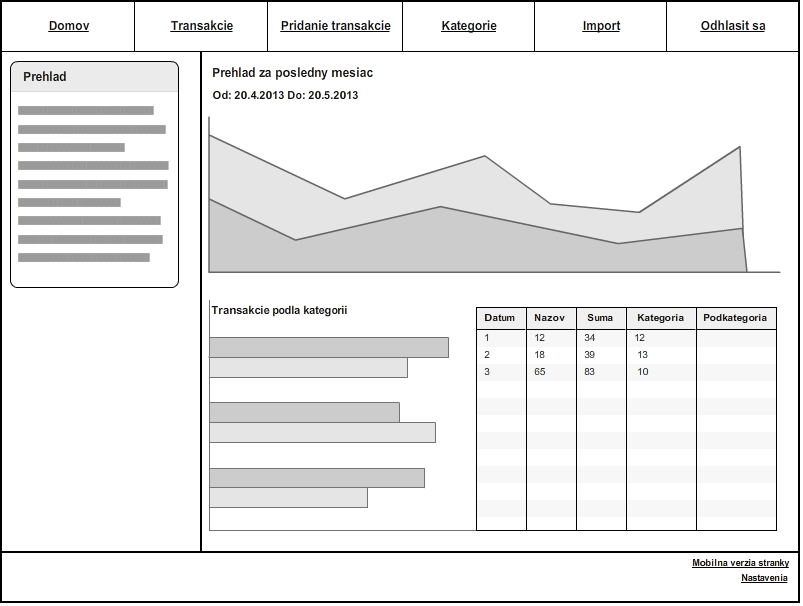
\includegraphics[width=11cm]{wireframe_home}
  \caption{wireframe - domov}
  \label{wireframe - domov}
\end{figure}  

Hneď pod ním sa nachádza ďalší graf zobrazujúci celkové sumy v rôznych kategóriách za rovnaké mesačné obdobie. Tento graf je má však len polovičnú šírku vrchného grafu a tak sa vedľa neho zmestil aj tabuľkový rozpis posledných transakcií aj s možnosťou stránkovania a usporiadania podľa rôznych stĺpcov. Ako som už v úvode naznačil, všetky tieto informácie uvidí používateľ bez nutnosti skrolovania. Pôvodne som chcel tieto informácie s kategóriami zobrazovať v koláčovom grafe. Po dohode s pánom školiteľom som od toho upustil, pretože použitý graf je prehľadnejší a v koláčovom grafe ma človek väčší problém porovnať uhly a zistiť ktorý je väčší. Pri aktuálnom grafe to je možné rozpoznať ihneď.


\subsubsection{Transakcie}
Hlavným zámerom tejto stránky je používateľovi sprostredkovať prehľad vo všetkých transakciách a grafické porovnanie príjmov a výdavkov v určitom období. Pod navigáciu som umiestnil graf podobný tomu z domovskej stránky. Obsahuje však niekoľko rozdielov. Príjmy aj výdavky sú v ňom zobrazované do plusových hodnôt. Tým je zjednodušené ich porovnávanie. Narozdiel od krivky s priebežnou bilanciou sa tu nachádza rozdielová krivka. Pri každom dni, prípadne mesiaci alebo roku, zobrazuje rozdiel príjmov výdavkov. Ak teda v určitý deň(mesiac, rok) presiahne suma výdavkov sumu príjmov, tak bude táto krivka v mínusových hodnotách. 
\begin{figure}[ht]
  \centering
      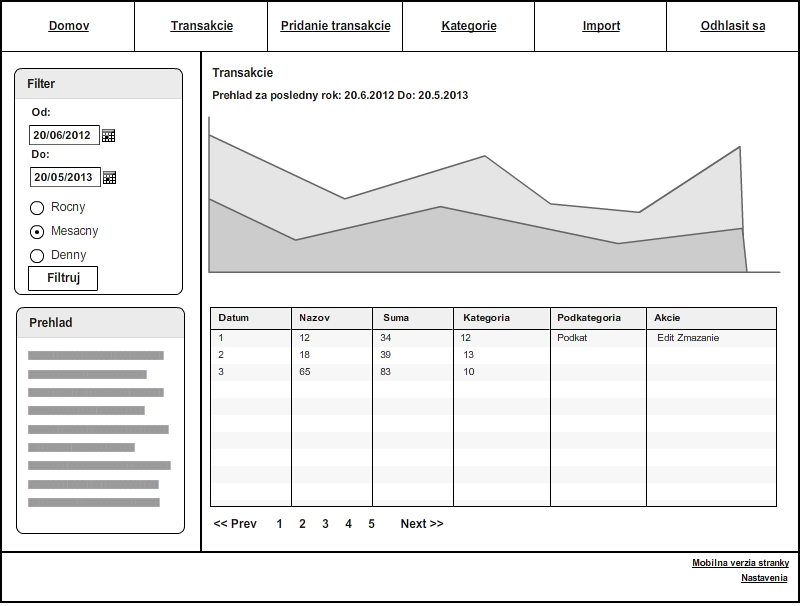
\includegraphics[width=11cm]{wireframe_transakcie}
  \caption{wireframe - transakcie}
  \label{wireframe - transakcie}
\end{figure} 

Pod grafom sa nachádza tabuľka s rozpisom transakcií. Okrem údajov ktoré ponúka podobná tabuľka z domovskej stránky obsahuje táto naviac aj tlačidlá s akciami, ktoré sa dajú použiť pri každej transakcii. Ide o editovanie transakcie, vymazanie transakcie a posledným je vymazanie vybratej transakcie a zároveň všetkých jej ďalších opakovaní  v budúcnosti. Jej predchádzajúce opakovania zostanú uložené.

Všetky údaje pre grafy a transakcie je možné filtrovať pomocou ponuky v ľavej časti stránky. Používateľ si vyberie časový rozsah od-do a rozdelenie v grafe podľa rokov, mesiacov alebo dní.


\subsubsection{Pridanie transakcie}
Jednoduchá stránka na pridávanie transakcií. Používateľ vyberá typ transakcie(príjem alebo výdavok). Názov transakcie, sumu, kategóriu, podkategóriu ktorá je zreťazená s kategóriou a dátum transakcie. Nakoniec má možnosť vybrať či pôjde o jednorazovú alebo opakovanú transakciu. Pri vybratí opakovanej sa mu zobrazia ďalšie možnosti. Interval opakovania a počet opakovaní. V tomto prípade sa vytvorí jedna pôvodná transakcia a ďalšie jej opakovania, ktoré budú v obsahovať pole \texttt{original\_transaction\_id} s \texttt{id} ich pôvodnej transakcie.
\begin{figure}[ht]
  \centering
      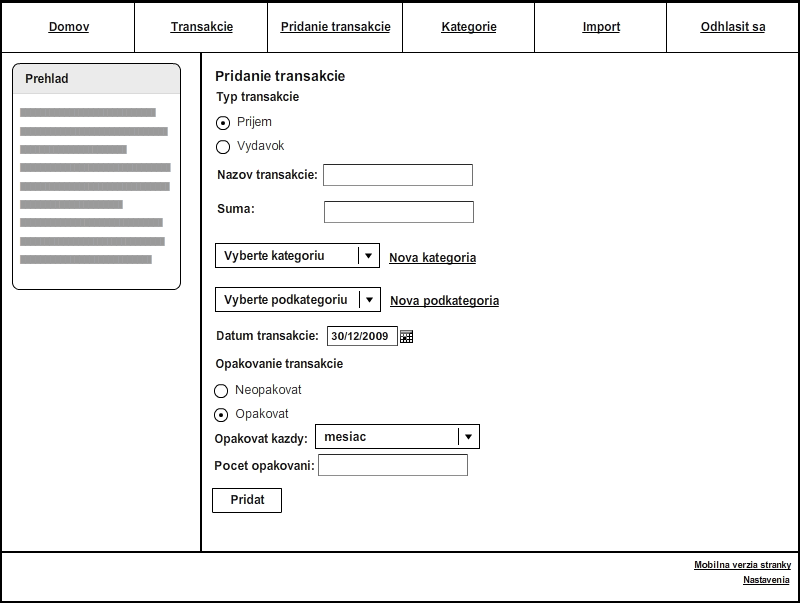
\includegraphics[width=11cm]{wireframe_add}
  \caption{wireframe - pridanie transakcie}
  \label{wireframe - pridanie transakcie}
\end{figure}
 

\subsubsection{Kategórie}
Základný graf na tejto stránke zobrazuje príjmy a výdavky podľa kategórií za vybraté obdobie pomocou filtra. Prednastavené obdobie je rok dozadu od aktuálneho dátumu. Pod ním sa nachádza tabuľkový výpis transakcií ako na stránke \emph{Transakcie}. Na tejto stránke je taktiež možné použiť filter na rozsah dátumov od-do. Pri vybratí konkrétnej kategórie je používateľovi zobrazený graf kategórie v čase. Tento graf je tiež možné filtrovať. V spodnej časti stránky sú vtedy zobrazené aj podkategórie ktoré patria do vybranej kategórie.
\begin{figure}[ht]
  \centering
      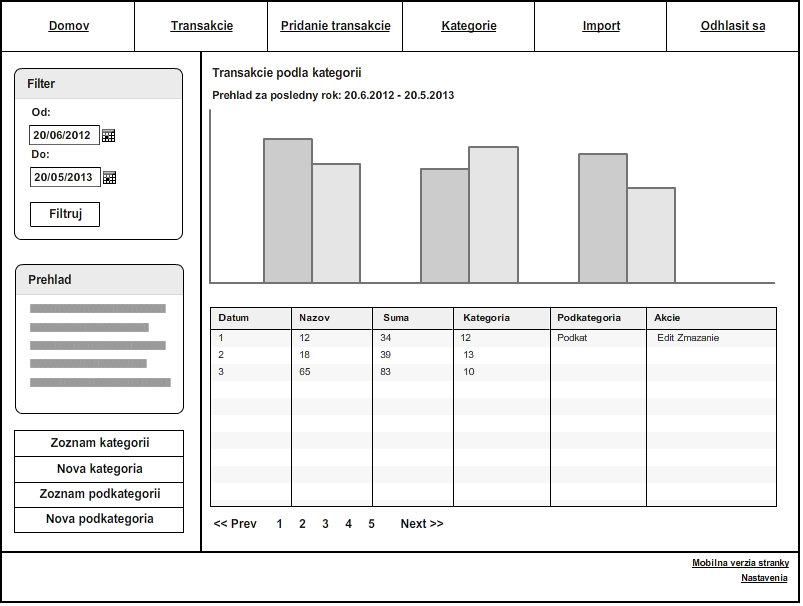
\includegraphics[width=11cm]{wireframe_kategorie}
  \caption{wireframe - kategorie}
  \label{wireframe - kategorie}
\end{figure} 

Po vybratí podkategórie sa zobrazí používateľovi informácia o nadradenej kategórii a taktiež tabuľka so všetkými transakciami, ktoré patria do tejto podkategórie. Samozrejmosťou sú tlačidlá s akciami, ktoré je možné aplikovať na vybratú podkategóriu. Ide o mazanie a editovanie a nachádzajú sa v ľavej časti stránky. 



\subsubsection{Import}
Stránka import poskytuje používateľovi tabuľkový prehľad importovaných výpisov z banky. Pri každom výpise sú na výber akcie spracovať, editovať a vymazať výpis. Najdôležitejšia akcia je spracovanie výpisu. Spracovanie výpisu podporuje aktuálne len výpisy Slovenskej Sporiteľne vo formáte ABO. Importovaný výpis z banky je spracovaný a používateľ dostane stránku s dodatočnou možnosťou upraviť kategórie a podkategórie každej transakcie z importovaného výpisu.

\subsubsection{Nastavenia}

Základné nastavenia účtu používateľa. Na tejto stránke si má používateľ možnosť zmeniť meno, priezvisko alebo môže požiadať o zmenu svojho hesla. Z dôvodu zvýšenej bezpečnosti mu bude potom zaslaný email s resetovacím odkazom. Vzhľadom k tomu, že táto ponuka nastavení nebude veľmi často využívaná, umiestnil som odkaz s ňou na spodnú časť stránky do pätičky. 

\subsubsection{Odhlásiť sa}

Používateľ je po kliknutí odhlásený z aplikácie, zároveň je zrušená jeho session a je presmerovaný na prihlasovaciu stránku.

\subsection{Mobilné rozhranie}
Pre zjednodušenie ovládania aplikácie na mobilných zariadeniach som pracoval aj na mobilnom rozhraní. Veľmi nápomocnou mi v tomto bola knižnica jQuery Mobile \cite{jQueryMobile}\, ktorá mi pomohla okrem funkčnosti aj s grafickým prevedením aplikácie vďaka jej základnému css layoutu pre mobilné prehliadače. Navigáciu som pri tomto rozhraní presunu spodnú časť stránky, tak ako to býva zvykom pri mobilných zariadeniach. Pokiaľ nie je potrebná tak sa automaticky zroluje, aby bola využitá maximálna plocha a mohlo byť zobrazených čo najviac informácií. V tejto spodnej časti stránky sa nachádza aj tlačidlo na prepnutie na plnú verziu stránky a taktiež aj tlačidlo na odhlásenie sa z aplikácie. 

Pre zachovanie prehľadnosti a jednoduchosti ovládania som počet odkazov v navigácii znížil na základné 4, ktoré ďalej opíšem trochu podrobnejšie. 

\subsubsection{Domov}
Základná stránka aplikácie, ktorú uvidí používateľ po prihlásení. Zobrazuje prehľadnú aktuálnu bilanciu financií používateľa. Je to ten istý prehľad ktorý nájde používateľ v plnom webovom rozhraní  vľavo pod navigáciou. Pod touto bilanciou sa nachádza graf transakcií podľa kategórií. V tomto grafe sú zarátané transakcie za posledný mesiac. Pod ním je prehľadná tabuľka s transakciami. Zobrazuje dátum, názov, sumu a kategóriu do ktorej je zaradená konkrétna transakcia. Graf zobrazujúci transakcie za určité obdobie som vynechal. Vzhľadom na malé rozlíšenie by nemal dostatočne dobrý informatívny charakter.
\subsubsection{Transakcie}
Prehľadný tabuľkový zoznam transakcií za posledný mesiac. Možnosť triedenia podľa rôznych stĺpcov je samozrejmosť. Každá transakcia zobrazuje svoj dátum, názov, sumu, kategóriu a podkategóriu. Na rozdiel od zoznamu na domovskej stránke je pri transakcii aj možnosť jej úpravy, zmazania. Taktiež sa tu nachádza aj možnosť zmazania vybranej transakcie a zároveň aj všetkých jej budúcich opakovaní.

Pod touto tabuľkou je umiestnené filtrovacie menu, ktoré som opisoval už pri webovom rozhraní.
\subsubsection{Pridanie transakcie}
Pridávanie transakcie je nastaveniami zhodné s pridávaním transakcie v plnom webovom rozhraní. Upravený je len dizajn tak aby vyhovoval mobilným zariadeniam.
\subsubsection{Kategórie}
Stránka kategórie zobrazuje graf príjmov a výdavkov podľa kategórií za posledný rok. Pod grafom za nachádza rozpis týchto kategórií s podrobnými informáciami o každej z nich tak ako je to aj na stránke \emph{Transakcie}. 


\section{Objektový model}
\subsubsection{Transactions}
Pre aplikáciu Domáce účtovníctvo sú najdôležitejšou časťou transakcie. Rovnako je pre objektový model najvýznamnejšia trieda \texttt{transactions}. Táto trieda uchováva informácie o všetkých transakciách. Transakcie sú rozdelené na príjmy a výdavky podľa \texttt{transaction\_type\_id} a preto na ne nie sú nutné 2 špeciálne triedy. Každej transakcii je okrem jej typu priradená aj jej kategória, podkategória, id používateľa ktorému patrí a informácia či ide o transakciu ktorá sa opakuje. Takisto má každá transakcia svoj názov, sumu a dátum kedy prebehla.
\subsubsection{Users}
Druhou významnou triedou sú používatelia, ktorí sú reprezentovaní v triede \texttt{users}. Nájdeme v nej všetky informácie týkajúce sa používateľa. Zaujímavá je položka \texttt{active}. Určuje či je používateľ stále aktívny a má prístup do systému. V prípade zrušenia konta sa zmení len táto položka a tým je používateľovi zablokovaný ďalší prístup do aplikácie. Každý zaregistrovaný používateľ je zatriedený do jedného z dvoch typov. Môže ísť o admina alebo o bežného používateľa. Každý používateľ môže mať viacero svojich transakcií, kategórií, podkategórií a výpisov.
\subsubsection{Categories}
Trieda obsahujúca informácie o kategóriách transakcií. Každá kategória patrí určitému svojmu používateľovi. Kategória má minimálne jednu svoju podkategóriu.
\subsubsection{Subcategories}
Trieda obsahujúca informácie o podkategóriách. Každá podkategória patrí svojmu používateľovi a taktiež aj svojej nadradenej kategórii.
\subsubsection{User\_types}
Trieda \texttt{user} types slúži na identifikáciu a pomenovanie typu používateľa. Aktuálne sú možné 2 typy používateľov. Admin a bežný používateľ.
\subsubsection{Transaction\_types}
Trieda \texttt{transaction\_types} slúži na identifikáciu a pomenovanie typu transakcie. Tie sú rozdelené na príjmy a výdavky.
\subsubsection{Imports}
Trieda, ktorá obsahuje informácie o importoch používateľa. Každý import patrí svojmu konkrétnemu používateľovi.



\chapter{Implementácia}

TODO MAYBE
info napr o domovskej stranke ...v akom controlleri je atd, ako cake implementuje controller .. ako som includoval controller do ineho

Mojim hlavným cieľom v implementácii bolo využiť nadobnuté vedomosti z programovania weboských aplikácií a skĺbiť ich s vedomosťami a funkcionalitou ktorú ponúka MVC framework CakePHP. S generovaním prehľadných grafom mi pomohla implementácie pluginu \texttt{HighCharts}. 

\section{CakePHP}
Základná implementácia vo frameworku CakePHP je na princípe toho, že každá trieda z tabuľky má svoj vlastný \texttt{controller}, \texttt{model} a rôzne prislúchajúce \texttt{views}. Tento princíp som využíval aj ja. V každom controllery som si definoval potrebné funkcie, nazývané aj akcie tohto controllera. 

\subsection{AppController}
Všetky mnou vytvorené controllery rozširujú možnosti preddefinovanej triedy \texttt{AppController} a tá možnosti základnej triedy \texttt{Controller}. V triede \texttt{AppController} som si definoval všetky potrebné akcie, triedy a komponenty CakePHP, ktoré budem chcieť používať v ostatných mnou vytvorených controlleroch. U mňa to boli triedy \texttt{CakeTime}, \texttt{CakeEmail}(nahrádza \texttt{EmailComponent} zo starších verzií cakePHP), komponenty \texttt{Auth}, \texttt{Session} a \texttt{Cookie}. Zadefinoval som tu taktiež aj \texttt{layout} pre webové a mobilné rozhranie.

Hlavná a veľmi dôležitá funkcia v \texttt{AppController} je verejná funkcia \texttt{beforeFilter}. Dávajú sa do nej akcie ktoré sú volané ako prvé a ešte pred akciou controllera. Sú to napríklad akcie súvisiace s autorizáciou používateľa a jeho oprávnení. Taktiež v nej kontrolujem prístup z mobilného zariadenia a s tým súvisiace neskoršie prepnutie na mobilný vzhľad aplikácie.

Ďalšou funkciou je \texttt{afterFilter}, ktorá je zavolaná až po akcii controllera a renderovaní \texttt{view}. Skontroluje či bol v \texttt{beforeFilter} zistený prístup z mobilného zariadenia a nastaví príslušný mobilný vzhľad. Pokiaľ je vytvorené, tak nastaví aj špecifické mobilné \texttt{view}.


\subsection{TransactionsController}
Základom aplikácie Domáce účtovníctvo je práca s transakciami a preto je práve \texttt{TransactionsController} najzaujímavejším a najdôležitejším controllerom. Zaoberá sa spracovaním transakcií a tvorbe prehľadných grafov a tabuľkových prehľadov. Už skôr som spomínal, že na tvorbu grafov používam Highcharts plugin. Preto bolo jednou z prvých vecí pridanie komponentu \texttt{HighCharts.HighCharts} do tohto controllera. Používam ho v každej akcii v ktorej generujem grafy. 

\section{Dáta pre HighCharts grafy} 
Základom každého grafu sú dáta. V mojich grafoch potrebujem naplniť hodnotami polia pre X-ové súradnice a polia pre Y-ové súradnice. Napríklad na domovskej stránke zobrazuje vrchný graf na X-vej súradnici dni za posledný mesiac a na y-ovej sumy transakcií za tieto konkrétne dni. Polí s x-ovými súradnicami môže byť aj viac. Zaleží to podľa počtu údajov ktoré chcem zobrazovať. Napríklad na spomenutej domovskej stránke je v jednom grafe stĺpcový prehľad príjmov, stĺpcový prehľad výdavkov a krivka priebežnej bilancie. Pod grafom sa nachádzajú tlačidlá s možnosťou zobrazenia len niektorého z týchto údajov. 

Jednou zo zložitejších častí implementácie týchto grafov bolo správne prednastavenie polí s dátami a nulovými hodnotami. Je to spôsobené tým, že nie každý deň musí byť pridaná určitá transakcia. Preto pokiaľ som nechcel, aby mi z grafu vypadli dni bez transakcií, musel som si po vybratí rozsahu dátumov vo filtry nastaviť nulové hodnoty pre každý deň, prípadne mesiac alebo rok. Najzložitejšie sa to implementovalo pri dennom filtry. Najjednoduchši prípad bol ak bol rozsah dní len v strede určitého mesiaca. Pokiaľ rozsah prekračoval mesiac potreboval som dĺžky všetkých mesiacov ktoré rozsah zahŕňal. Ak rozsah prekročil rok, tak sa príprava dát sťažila ešte viac. Pri filtrovaní dní som takto získaval až trojrozmerné polia naplnené nulovými hodnotami. Až potom som ich mohol naplniť dátami z reálnych transakcií.




\section{Stránkovanie a grafy transakcií}
Pokračujem opisom domovskej stránky. Pod grafom sa nachádza tabuľka s prehľadom všetkých transakcií za tento posledný mesiac. Na tvorbu týchto tabuliek som využil komponent \texttt{PaginatorComponent}. Ide o veľmi dobre spracovaný komponent, ktorý ponúka CakePHP na tvorbu dotazov na databázu. Ponúka možnosť stránkovania a triedenia podľa stĺpcov tabuľky. 
\begin{lstlisting}
$this->paginate = array(
	'limit' => 20,
	'order' => array(
			'Transaction.post_date' => 'asc'
	),
	'conditions' => array(
			'Transaction.user_id' => $this->Session->read('User.id'),
			'Transaction.post_date >=' => $filterdata['from_date'],
			'Transaction.post_date <=' => $filterdata['to_date'],
	),
); 
\end{lstlisting}
Ako je možné vidieť v ukážke kódu, najčastejšie sa v ňom nastavujú 3 možnosti. Limit výpisov na jednu stránku, základné zoradenie týchto výpisov a podmienky výberu. V mojom prípade som nastavil limit 20 transakcií na jednu stránku, triedenie podľa dátumu transakcie a výber transakcií patriacich aktuálne prihlásenému používateľovi v rozsahu od a po určitý dátum. Framework si vďaka takémuto nastaveniu vybral všetky potrebné dáta s transakciami. Pôvodne som používal tieto dáta vybraté cez \texttt{paginate} aj pre grafy. Zistil som však, že dáta boli vybraté vždy len pre konkrétnu stránku zo stránkovania a tak sa mi na grafe vygenerovala napríklad len polovica údajov. Keď som chcel ďalšie, bolo potrebné prejsť na druhú stránku v stránkovaní. Vyriešil som to tak, že dáta pre grafy som získaval pomocou funkcie find. Tak som sa dostal ku všetkým potrebným dátam bez toho aby boli obmedzené stránkovaním.  

Ďalší problém, ktorý sa vyskytol, bol pri použití filtra od/do a prepínania stránkovania. Ak používateľ použije filter pre výber rozsahu dátumov transakcií a rozdelenia týchto transakcií, zmení týmto údaje zobrazované v grafe a taktiež aj v tabuľke. Ak však potom klikne na inú stránku v stránkovaní, tieto údaje sa stratili a boli nahradené tými pôvodnými. Riešením bolo použitie Session. Po nastavení filtra som údaje z neho uložil do Session. Vďaka tomuto riešeniu sa pri stránkovaní nestratili a mohol som ich používateľovi prednačítať aj v iných častiach aplikácie, kde bola možnosť filtrovať dáta pre zobrazenie v grafoch a tabuľke.

\section{Spracovanie výpisov}
Jednou z ďalších zaujímavých a zložitých prvkov aplikácie bolo nahrávanie a spracovanie výpisov. Aktuálna verzia aplikácie podporuje spracovanie výpisov Slovenskej sporiteľne, ktorá ich poskytuje v zaužívanom formáte ABO. Na pochopenie tohoto ABO výpisu som si najskôr musel naštudovať štruktúru jeho výpisu. 

Celý súbor výpisu sa skladá z 2 typov viet. Prvá veta je typu 074. Je to hlavička výpisu z účtu ktorá má fixnú dĺžku 114 znakov. Druhá veta je typu 075. Označuje údajovú položku výpisu z účtu. Jej fixná dĺžka je 128 znakov. Podrobnejšia štruktúra týchto viet zaberá 2 strany a preto ju tu celú nebudem opisovať. Zaujímavosťou v tomto výpise je, že jednotlivé pozície čísla účtu v tomto výpise sú pozmenené. Napríklad pre číslo účtu 0123456789 je číslo účtu v ABO výpise v tvare 9785012346. Takto vyzerá ukážka spracovania tohto čísla účtu:
\begin{lstlisting}
$cislo_uctu_partnera = substr($lines[$i], 3, 10);  // nacitanie cisla uctu zo spravnej pozicie udajovej polozky vo vypise
$cislo_uctu_decoded = substr($cislo_uctu_partnera, 4, 5) . substr($cislo_uctu_partnera, 3, 1) . substr($cislo_uctu_partnera, 9, 1) . substr($cislo_uctu_klienta, 1, 2) . substr($cislo_uctu_partnera, 0, 1);  // zlozenie cifier cisla uctu do spravneho poradia 
$predcislie_uctu_partnera = substr($lines[$i], 13, 6);  // nacitanie predcislia uctu
$parsed_file['content'][$i]['account_number'] = $cislo_uctu_decoded;  // priradenie cisla uctu do pola
$parsed_file['content'][$i]['account_prefix'] = $predcislie_uctu_partnera;  // priradenie predcislia uctu do pola
\end{lstlisting}


\section{Databázový model}
\subsubsection{Transactions}
Pre aplikáciu Domáce účtovníctvo sú najdôležitejšou časťou transakcie. Rovnako je pre databázový model najvýznamnejšia tabuľka \texttt{transactions}. Táto tabuľka uchováva informácie o všetkých transakciách. Transakcie sú rozdelené na príjmy a výdavky podľa \texttt{transaction\_type\_id} a preto na to nie je nutné 2 špeciálne tabuľky. \texttt{Transactions} obsahuje cudzie kľúče na stľpce v tabuľkách \texttt{transaction\_types}(\texttt{transaction\_\allowbreak type\_\allowbreak id}), \texttt{categories}(\texttt{category\_id}), \texttt{subcategories}(\texttt{subcategory\_id}), \texttt{users}(\texttt{user\_id}) a dokonca aj sama na seba. To využíva pri opakovaných transakciách odkazovaním na svoj stĺpec \texttt{original\_transaction\_id}.
\subsubsection{Users}
Druhou významnou tabuľkou sú používatelia, ktorí sú reprezentovaní v tabuľke \texttt{users}. Nájdeme v nej všetky informácie týkajuce sa použivateľa. Zaujímavá je položka active. Určuje či je používateľ stále aktívny a má prístup do systému. V prípade zrušenia konta sa zmení len táto položka a tým je používateľovi zablokovaný ďalší prístup do aplikácie. Táto tabuľka obsahuje jediný cudzí kľuč \texttt{user\_type\_id}, ktorý sa vzťahuje na stĺpec \texttt{id} v tabuľke \texttt{user\_types}. Ďalej je v tejto tabuľke zadefinovaný vzťah hasMany na tabuľky \texttt{transactions}, \texttt{categories}, \texttt{subcategories} a \texttt{imports}. Z toho vyplýva, že jednému používateľovi môže prislúchať viacero záznamov z týchto tabuliek.
\subsubsection{Categories}
Jednoduchá tabuľka obsahujúca informácie o kategóriách transakcií. Obsahuje len jeden cudzí kľúč \texttt{user\_id} na na stĺpec \texttt{id} v tabuľke \texttt{users}. 
\subsubsection{Subcategories}
Tabuľka obsahujúca informácie o podkategóriách. Na rozdiel od \texttt{Categories} obsahuje okrem cudzieho kľúča aj ďalší cudzí kľúč \texttt{category\_id} odkazujúci na kategóriu ktorej patrí.
\subsubsection{User\_types}
Tabuľka \texttt{user} types slúži na identifikáciu a pomenovanie typu používateľa. Aktuálne sú možné 2 typy používateľov. Admin a bežný používateľ.
\subsubsection{Transaction\_types}
Tabuľka \texttt{transaction\_types} slúži na identifikáciu a pomenovanie typu transakcie. Tie sú rozdelené na príjmy a výdavky.
\subsubsection{Imports}
Tabuľka obsahujúca len jeden cudzí kľúč \texttt{user\_id}, ktorý definuje vzťah \texttt{belongsTo} k tabuľke \texttt{user} a konkrétnemu používateľovi.
\begin{figure}[ht]
  \centering
      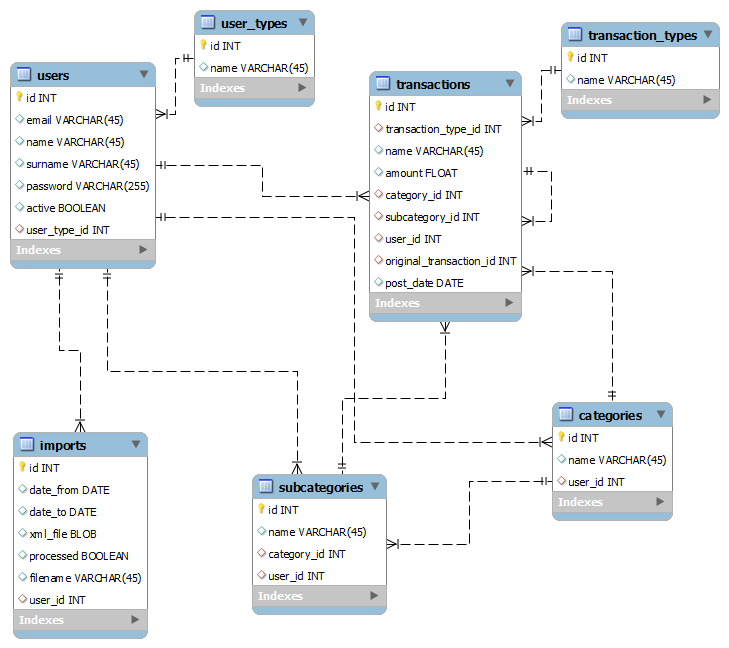
\includegraphics[width=15cm]{databazovy_model}
  \caption{Domáce účtovníctvo - Databázový model}
  \label{DataModel}
\end{figure}    


\section{Resetovanie hesiel}


\chapter{Záver}\label{chap:outro}
 
Zámerom mojej bakalárskej práce bolo vytvorenie prehľadnej aplikácie na správu domáceho účtovníctva. Hlavným cieľom bola webová aplikácia s plnou funkcionalitou. Od nej bola odvodená jednoduchšia mobilná verzia aplikácie. Vzhľadom na udržanie prehľadnosti a jednoduchosti používania tejto mobilnej aplikácie bola jej funkcionalita obmedzená len na najčastejšie používané funkcie.

Na začiatku práce som si spravil prehľad v podobných konkurenčných aplikáciách. Analyzoval som ich klady a zápory a do svojej aplikácie som sa pokúsil implementovať tie najlepšie riešenia z týchto rôznych aplikácií. Veľký dôraz som kládol na prehľadnosť a jednoduchosť ovládania aplikácie, pretože práve toto bola slabá stránka niektorých konkurenčných aplikácií. 

Ďalej som sa zaujímal o webové technológie, ktoré bude potrebné v práci použiť. Tu bolo jedným zo základných prvkov použitie frameworku CakePHP. Vďaka nemu, a MVC prístupu ktorý používa, sa programovanie aplikácie urýchlilo. Podstatnejšie však je, že sa jeho použitím sprehľadnil kód a zjednodušila prípadná budúca implementácia novej funkcionality. 

Po naštudovaní fungovania a začatia programovania s CakePHP bolo ďalším krokom vytvorenie prehľadných štatistických grafov. To som dosiahol pomocou pluginu HighCharts, ktorý slúži na tvorbu grafov. 

Jednou z finálnych častí práce bolo spracovávanie výpisov a následné vytvorenie transakcií z týchto výpisov. Vzhľadom k tomu, že skoro každá slovenská banka používa svoj vlastný formát výpisu, použil ten najuniverzálnejší vo formáte ABO. Ide o zaužívaný štandard bankových výpisov ktorý používa Slovenská sporiteľňa. 

Do budúcna by preto bolo dobré rozšíriť aplikáciu o spracovanie výpisov z iných bánk, prípadne o možnosť spravovania viacerých účtov používateľa v rámci jedného používateľského konta. Zaujímavým a pre používateľa motivačným rozšírením aplikácie by mohlo byť aj stanovenie si súkromných cieľov na ktoré by si financie postupne presúval a šetril. Táto aplikácia na báze MVC architektúry ponúka skutočne široké možnosti rozšírenia.

\backmatter

\nocite{*}
\bibliographystyle{abbrv}
\bibliography{literatura}


\newcommand{\dbappendix}[1]{\chapter{#1}}
\appendix
\dbappendix{Príloha}\label{appA}
{\large Priložené DVD médium}\\

Priložené DVD obsahuje:\\
\begin{itemize}
\item Text tejto práce vo formáte TEX a PDF
\item Zdrojové súbory aplikácie Domáce účtovníctvo:
	\begin{itemize}
		\item {\em nieco} - nieco
	\end{itemize}
\end{itemize}

\end{document}
